% Created 2023-10-22 Sun 21:05
% Intended LaTeX compiler: pdflatex
\documentclass[letterpaper, 11pt]{article}
              \usepackage{minted}
              \usepackage{lmodern} % Ensures we have the right font
\usepackage[T1]{fontenc}
\usepackage[utf8]{inputenc}
\usepackage{graphicx}
\usepackage{amsmath, amsthm, amssymb}
\usepackage[table, xcdraw]{xcolor}
\definecolor{bblue}{HTML}{0645AD}
\usepackage[colorlinks]{hyperref}
\hypersetup{colorlinks, linkcolor=blue, urlcolor=bblue}
\usepackage{titling}
\setlength{\droptitle}{-6em}
\setlength{\parindent}{0pt}
\setlength{\parskip}{1em}
\usepackage[stretch=10]{microtype}
\usepackage{hyphenat}
\usepackage{ragged2e}
\usepackage{subfig} % Subfigures (not needed in Org I think)
\usepackage{hyperref} % Links
\usepackage{listings} % Code highlighting
\usepackage[top=1in, bottom=0.25in, left=0.50in, right=0.50in]{geometry}
\renewcommand{\baselinestretch}{1.15}
\usepackage[explicit]{titlesec}
\pretitle{\begin{center}\fontsize{20pt}{20pt}\selectfont}
\posttitle{\par\end{center}}
\preauthor{\begin{center}\vspace{-6bp}\fontsize{14pt}{14pt}\selectfont}
\postauthor{\par\end{center}\vspace{-25bp}}
\predate{\begin{center}\fontsize{12pt}{12pt}\selectfont}
\postdate{\par\end{center}\vspace{0em}}
\titlespacing\section{0pt}{5pt}{5pt} % left margin, space before section header, space after section header
\titlespacing\subsection{0pt}{5pt}{-2pt} % left margin, space before subsection header, space after subsection header
\titlespacing\subsubsection{0pt}{5pt}{-2pt} % left margin, space before subsection header, space after subsection header
\usepackage{enumitem}
\setlist{itemsep=-2pt} % or \setlist{noitemsep} to leave space around whole list
\author{Bray Moll}
\date{\today}
\title{Homework 5}
\hypersetup{
 pdfauthor={Bray Moll},
 pdftitle={Homework 5},
 pdfkeywords={},
 pdfsubject={},
 pdfcreator={Emacs 29.1 (Org mode 9.6.6)},
 pdflang={English}}
\begin{document}

\maketitle


\section{1)}
\label{sec:orgd8c2685}
\subsection{Problem Setup}
\label{sec:org628190f}
\begin{minted}[,frame=single]{python}
import pandas as pd
from solver import solver
from solver import mesher
import plotnine as pn
\end{minted}

In this problem we are using a spatial domain
\(x \epsilon [0,1]\)

We are using an intial condition
\(T(x, t=0) = 0^\circ C\)
a left dirichlet boundary
\(T(0, t) = 50^\circ C\)

On the right size we will apply a zero Neuiman Boundary Condition
\(\frac{\partial T}{\partial x} (x = 1, t) = 0\)

We will set the thermal diffusivity to
\(\alpha ^2 = 0.0001 \frac{m^2}{s}\)

Additionally we can set paramaters of interest such as the maximum, the number of cells as well as the mesh type. The only difference for the mesh type in 1d is if the node is directly on the boundarys (as would be seen in the finite\textsubscript{difference} or if the edge cell face is on the boundary
\begin{minted}[,frame=single]{python}
def create_mesh(n_cells, mesh_type):
    mesh = mesher.create_1Dmesh(x=[0, 1], n_cells=n_cells, mesh_type=mesh_type)
    mesh.set_cell_temperature(0)  # set initial conditions to 0 celcicus
    mesh.set_dirichlet_boundary("left", 50)  # Left to 50 c
    mesh.set_neumann_boundary("right")
    mesh.set_thermal_diffusivity(0.0001)  # m^2/s
    return mesh

n_cells = 20
time_max = 30000

\end{minted}
\subsection{Explicit method Unstable}
\label{sec:orgeba8a31}
Create a solver object with time paramaters, desired method, and a mesh and solve using .solve(t\textsubscript{final})
\begin{minted}[,frame=single]{python}
explicit_solution_unstable = solver.solver_1d(
    mesh=create_mesh(n_cells, mesh_type),
    initial_time=0,
    time_step_size=15,
    method="explicit",
)
explicit_solution_unstable.solve(600)

\end{minted}

The data will be stored in a pandas data frame in the self.saved\textsubscript{data} atribute. For example, as we have 20 nodes, the first 20 rows will be the initial condition, followed by will be the first time step.


\begin{minted}[,frame=single]{python}
print(explicit_solution_unstable.saved_data.head(10))

\end{minted}

\begin{verbatim}
     method  time_step_size  time  x_cordinates  temperature
0  explicit              15     0      0.000000         50.0
1  explicit              15     0      0.052632          0.0
2  explicit              15     0      0.105263          0.0
3  explicit              15     0      0.157895          0.0
4  explicit              15     0      0.210526          0.0
5  explicit              15     0      0.263158          0.0
6  explicit              15     0      0.315789          0.0
7  explicit              15     0      0.368421          0.0
8  explicit              15     0      0.421053          0.0
9  explicit              15     0      0.473684          0.0
\end{verbatim}


The data can be plotted using your favorite tool for Pandas dataframes

\begin{minted}[,frame=single]{python}
time_points = [0,15,30,60,600]
plot_data_filterd_bool = explicit_solution_unstable.saved_data["time"].isin(time_points)
plot_data_filtered = explicit_solution_unstable.saved_data[plot_data_filterd_bool]

plot = (
    pn.ggplot(
        plot_data_filtered,
        pn.aes("x_cordinates", "temperature", color="factor(time)"),
    )
    + pn.geom_line()
    + pn.geom_point()
    + pn.facet_grid("method~time_step_size")


  )
plot.save("explicit_unstable.png")

\end{minted}

\begin{center}
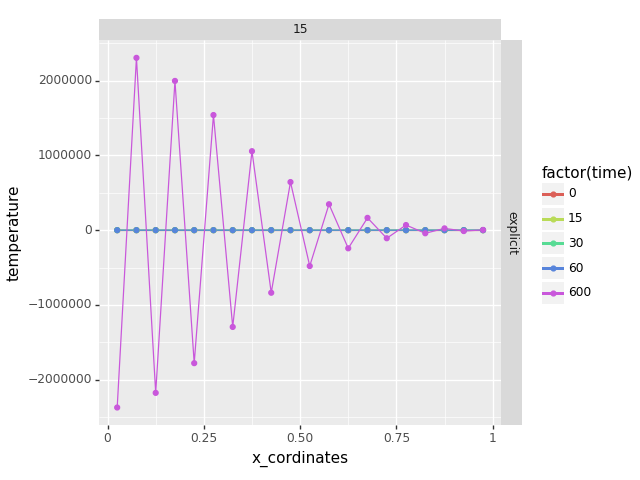
\includegraphics[width=.9\linewidth]{explicit_unstable.png}
\end{center}


As demonstrated, the explicit method will demonstrate numerical unstability when the time step it too large.


\subsection{Finite Difference Discritization}
\label{sec:org2e2bc44}
\begin{minted}[,frame=single]{python}
mesh_type = "finite_difference"
explicit_solution_stable = solver.solver_1d(
    mesh=create_mesh(n_cells, mesh_type),
    initial_time=0,
    time_step_size=1,
    method="explicit",
)
explicit_solution_stable.solve(time_max)

implicit_solution_15sec = solver.solver_1d(
    mesh=create_mesh(n_cells, mesh_type),
    initial_time=0,
    time_step_size=15,
    method="implicit",
)
implicit_solution_15sec.solve(time_max)

implicit_solution_1sec = solver.solver_1d(
    mesh=create_mesh(n_cells, mesh_type),
    initial_time=0,
    time_step_size=1,
    method="implicit",
)
implicit_solution_1sec.solve(time_max)

plot_data_finite_difference = pd.concat(
    [

        explicit_solution_stable.saved_data,
        implicit_solution_15sec.saved_data,
        implicit_solution_1sec.saved_data,
    ]
)
time_points = [
    0,
    15,
    30,
    60,
    600,
    3600,
    time_max,
]  # time points that you want to plot

plot_data_filterd_bool = plot_data_finite_difference["time"].isin(time_points)
plot_data_filtered = plot_data_finite_difference[plot_data_filterd_bool]

plot = (
    pn.ggplot(
        plot_data_filtered,
        pn.aes("x_cordinates", "temperature", color="factor(time)"),
    )
    + pn.geom_line()
    + pn.geom_point()
    + pn.facet_grid("method~time_step_size")

)

plot.save("finite_difference.png")


\end{minted}

\begin{center}
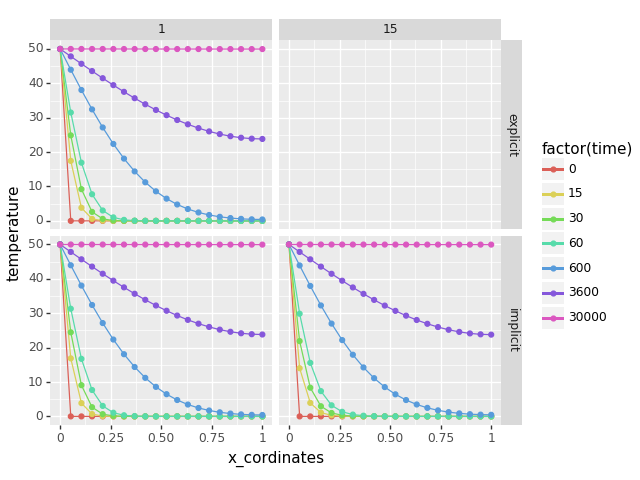
\includegraphics[width=.9\linewidth]{finite_difference.png}
\end{center}
\newpage

\subsection{Finite Volume Discritization}
\label{sec:orgc4eeb34}

Alternatly, the finite pvolume discritization can be used
\begin{minted}[,frame=single]{python}
mesh_type = "finite_volume"
\end{minted}

\begin{center}
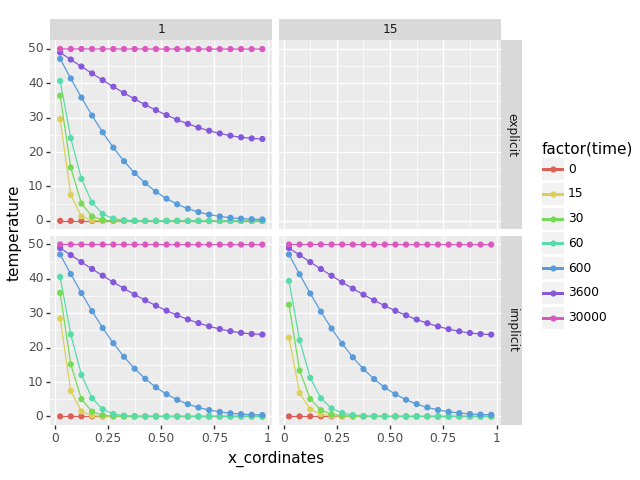
\includegraphics[width=.9\linewidth]{finite_volume.png}
\end{center}
\end{document}
